\chapter{Introduction}
\label{ch:Introduction}


According to \tcite{Li2009}, especially temperature and perceived temperature have a great impact on energy demand. Consequently, several authors combine forecasting energy time series using weather data. They mostly either focus on forecasting \gls{pv} electricity generation as in \tcite{Bofinger2006} and \tcite{Sperati2016} or on electricity generation from wind as in \tcite{Davo2016} and \tcite{Alessandrini2015}.\\

It is notable, that works using station-based data often try to do some sort of geographic interpolation to be able to obtain values for every possible position. Considering this thesis, there is no such problem, as the used grid-based data already provides such distributed values. Thus, when using grid-based data, the step of interpolation can be omitted, and therefore, less effort is required. Some works also regard only forecasting for specific locations or accumulated values for bigger areas. With grid-based data, more general predictions can be made regarding the target location, as there is no binding to a certain locality.\\

Another interesting point is, that the works that forecast weather related time series all used grid-based data, though some of them also used station-based data to refine their forecasts. Among the papers that aimed for forecasting power or similar often only station-based data is used which leads to the assumption that less effort has been made in these fields, as it is still more complex to acquire grid-based data. However, there remains the possibility that station-based data is more suitable, even though this means a trade-off in terms of flexibility. Of course it is also possible that this has to do with the fact, that there is no grid-based power data available as this may harm privacy issues.\\

%Your thesis should start with an introduction. The introduction is supposed to motivate your thesis.
%Discuss the relevance of your topic, why are you looking into it, why is it relevant in the field? Cite important research related to your motivation.
%Briefly state the problem as in the abstract and repeat the contribution, for example in the form of research questions. 

%Give an outline of your thesis.


%Below, you will find an example figure (\Cref{fig:example}). Please use the caption of your figures to describe everything in the figure, additionally to what you have written about the figure in the text. Everyone should be able to understand the figure just reading its caption.

%\begin{figure}[h!]%
%\centering
%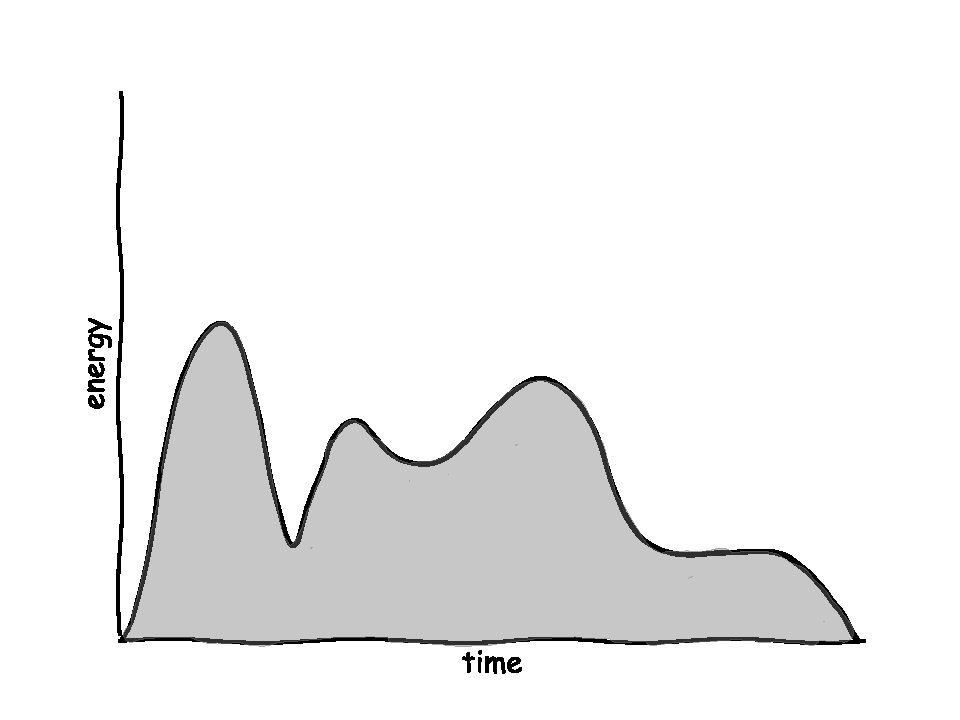
\includegraphics[width=0.5\columnwidth]{plots/Figure_2_demand}%
%\caption{This is an example figure. It shows a fictional demand of energy (in grey) over time.}%
%\label{fig:example}%
%\end{figure}

%This work is supposed to refer about including grid-based data into load forecasts using different methods.\\
